\documentclass{tfgitic}[2023/07/07]
% per a fórmules químiques
\usepackage[version=4]{mhchem}
% Per dibuixar gràfics: base general i gràfics senzills
\usepackage{tikz}
\usetikzlibrary{arrows, positioning, automata}
\tikzset{initial text=Inici, every state/.style={thick, fill=gray!10}}
% Per dibuixar gràfics: circuits electrònics
\usepackage[europeanresistors,americaninductors]{circuitikz}
% Per dibuixar gràfics: diagrames diversos
\usepackage{pgfplots}
% Per escriure algoritmes
\usepackage[plain,figure]{algorithm2e}
% Per a usar taules elàstiques
\usepackage{tabularx}

% Indica quines bd bibliografiques usarem
\addbibresource{tfg.bib}

% Marges en els algoritmes
\setlength{\algomargin}{4em}

% Versió de pgfplots a usar
\pgfplotsset{compat=newest}

\definecolor{tufte1}{rgb}{0.7,0.7,0.55}
\definecolor{yellowmarker}{HTML}{DEF440}

\pgfplotsset{
	tufte bar/.style={
		ybar,
		axis line style={draw opacity=0},
		xtick=\empty,
		ymin=0,
		bar width=3mm,
		x=2*\pgfkeysvalueof{/pgf/bar width},
		ymajorgrids,
		grid style=white,
		axis on top,
		major tick length=0pt,
		cycle list={
			fill=tufte1, draw=none\\
		},
		enlarge x limits={
			abs=0.5*\pgfkeysvalueof{/pgf/bar width}
		},
		axis x line*=bottom,
		x axis line style={
			draw opacity=1,
			tufte1,
			thick
		},
		yticklabel=\pgfmathprintnumber{\tick}\,\%
	}
}

% Bits en plural
\DeclareSIUnit{\bits}{bits}
% Elimina els zeros sobrants en decimals
\sisetup{zero-decimal-to-integer}

\title{OsPlot: Com implementar osci\l.loscopis amb un microcontrolador i Linux}

\subtitle{Una guia pràctica per a la creació d'un osci\l.loscopi digital amb plataformes obertes}

\author{Joan Vilardaga Castro}

\advisor{Francisco del Águila López}

\begin{acknowledgments}
Vull expressar el meu més sincer agraïment a la meva família,
especialment als meus estimats pares, per donar-me l'oportunitat
d'obtenir una educació i per donar-me suport incondicional en aquesta
etapa de la meva vida. Sense ells, aquest treball no hauria estat
possible.

També desitjo expressar el meu reconeixement a alguns dels meus
professors que han tingut un paper fonamental en la meva formació
acadèmica. A na Maria Antònia i en Carmelo, professors de secundària,
els estic profundament agraït per la seva dedicació i per despertar en
mi la passió per la informàtica i l'electrònica. I als professors de
la universitat, na Rosa, en Sebas i en Xavier, vull agrair-los per la
seva guia, el seu suport i els seus coneixements compartits durant el
meu recorregut universitari.

Menció especial a en Francisco, el meu tutor d'aquest Treball de Fi de
Grau. Li estic profundament agraït per la seva idea que ha permès
l'existència d'aquest treball, així com les seves aportacions durant
el desenvolupament d'aquest.
\end{acknowledgments}

\begin{resum}
En aquest document es descriu una guia que permeti a qualsevol persona
transformar un microcontrolador i un ordinador en un osci\l.loscopi
funcional. Mitjançant l'ús de plataformes obertes com Linux, Arduino i
GNUPlot, aquesta investigació intenta oferir una solució de baix cost
i accessible per a gent interessada en l'anàlisi de senyals.
\end{resum}

\begin{abstract}
\begin{otherlanguage}{english}
This document describes a guide that enables anyone to transform a
microcontroller and a computer into a functional oscilloscope. By using
open platforms such as Linux, Arduino and GNUPlot, this research aims
to provide a low-cost and accessible solution for people interested in
signal analysis.
\end{otherlanguage}
\end{abstract}

\begin{document}

\chapter{Introducció}
\label{cap:intro}

\section{Origen del treball: Osci\l.loscopi amb GNUPlot}
\label{sec:origen}

GNUPlot \cite{gnuplot} és un programa de traçat de gràfics en 2D i 3D
que permet visualitzar i analitzar diferents conjunts de dades. Tot i
que GNUPlot és una eina per fer gràfics estàtics, es pot combinar amb
altres programes o \est{scripts} per aconseguir la funcionalitat de
traçat en temps real.

És precisament aquest descobriment el que obre la porta a la
possibilitat de fer un osci\l.loscopi amb GNUPlot com a plataforma
principal. Així, aquesta investigació s'enfoca a preparar una guia que
permeti crear un osci\l.loscopi digital mitjançant GNUPlot.

\section{Objectius}
\label{sec:objectius}

\begin{enumerate} 
	\item Evaluar la capacitat de GNUPlot per visualtizar dades en
          temps real.
	\item Desenvolupar una guia per OsPlot, una arquitectura genèrica
          que pot transformar un microcontrolador i un ordinador en
          un osci\l.loscopi.
  \item Estendre l'arquitectura amb alternatives a GNUPlot.
	\item Implementar programes de referència que explotin les
          diferents possibilitats de l'arquitectura.
\end{enumerate}

\section{Com funciona un osci\l.loscopi}
\label{sec:com-funciona-oscil·loscopi}

Un osci\l.loscopi \cite{viqui-oscil·loscopi} és un instrument de
mesura que s'utilitza per visualitzar i analitzar senyals elèctrics
variables en el temps. Com amb moltes altres coses, els
osci\l.loscopis són instruments que han evolucionat amb la
digitalització, creant una nova generació d'osci\l.loscopis més
precisos i que poden fer operacions molt més complexes com mitges, pic
a pic o transformades ràpides de Fourier.

\subsection{Funcionament bàsic}
\label{subsec:funcionament-bàsic}

Els osci\l.loscopis digitals es basen en l'ús d'un \acro{ADC}
(convertidor analògic-digital), un sistema que converteix senyals
analògics en senyals digitals, les quals es processen per generar una
representació gràfica en temps real a la pantalla. L'eix horitzontal
indica el temps, i l'eix vertical indica generalment voltatge (tot i
que es poden mesurar altres magnituds com el corrent).

Tots els osci\l.loscopis incorporen un subsistema de \est{trigger}
\cite{funcionament-trigger} que té com a funció establir un punt de
referència i sincronitzar la captura de les dades. Aquest subsistema
és essencial per garantir una visualització estable i repetible. Sense
el \est{trigger}, el senyal a visualitzar es desplaçaria constantment
a través de l'eix horitzontal, fent impossible la seva observació.

\subsection{Conceptes importants de senyals digitals}
\label{subsec:conceptes-pds}

Com que el treball se centra en osci\l.loscopis digitals, és necessari
conèixer alguns dels conceptes claus del processament digital del
senyal \cite{llibre-pds}:

\begin{itemize}
	\item Senyal analògic (o continu): Tipus de senyal format per
          variables contínues. Encara que aquests valors estiguin
          confinats en un rang màxim i mínim, poden tenir una precisió
          infinita, no hi ha espais buits.
	\item Senyal digital (o discret): Seqüència de valors discrets
          separats en el temps. A diferència dels analògics, els
          senyals discrets tenen espais buits.
	\item Quantització: És el procés d'aproximar un valor continu
          al valor discret més proper. Sigui aproximació o truncament,
          sol introduir error de mesura, ja que un valor discret no
          pot representar els infinits decimals d'un valor continu.
	\item Resolució: És la diferència entre dos valors d'un rang
          discret. Determina el màxim error de discretització i el
          nombre de bits d'una mostra.
	\item Mostreig: Procés que transforma un senyal analògic en un
          senyal discret mitjançant l'ús repetit de la quantització.
          Cada valor quantitzat és una mostra del senyal analògic.
	\item Freqüència de mostreig: El nombre de mostres que captura
          un \acro{ADC} cada segon. La màxima freqüència que podrà
          captar l'osci\l.loscopi serà com a màxim la meitat de la
          freqüència de mostreig (criteri de Nyquist).
\end{itemize}

\chapter{OsPlot}

En aquest capítol primer s'explorarà la manera de convertir GNUPlot en
una eina per visualitzar dades en temps real. Seguidament, s'intentarà
dissenyar l'arquitectura més simple d'OsPlot, on una Arduino envia pel
port sèrie mostres d'un byte, i GNUPlot les representa gràficament. I
finalment s'analitzaran les dues vies possibles per desenvolupar un
osci\l.loscopi amb sistema de \est{trigger}, i s'intentarà ampliar al
màxim les arquitectures proposades.

\section{Visualització en temps real amb GNUPlot}

Per tal de transformar GNUPlot en una eina que pugui simular un
osci\l.loscopi, primer s'ha d'aconseguir una visualització en temps
real de les dades. Com s'ha mencionat a l'introducció, GNUPlot és una
eina per graficar que està dissenyada per llegir fitxers de dades
estàtics.

De fet, GNUPlot només pot generar un gràfic a partir d'un conjunt de
dades si s'arriba a la condició de final de fitxer (\acro{EOF}). Tot i
que el port sèrie pot fer saltar la condició d'\acro{EOF} (amb el
caràcter \acro{EOT}, 0x04), fer-ho reiniciaria l'Arduino cada cop que
GNUPlot obre el ``fitxer'' del port sèrie. Per tant, es requereix un
programa auxiliar que mantingui obert el flux de dades amb el
microcontrolador, i que alhora pugui generar la condició d'\acro{EOF}
per a la lectura de dades.

En aquesta secció es detallarà la implementació d'aquest programa
auxiliar per establir una comunicació estable i permetre la
visualització en temps real de les dades en el gràfic de GNUPlot.

\subsection{Reescriptura contínua del fitxer}

En un primer moment, es pot pensar que la solució per aconseguir que
GNUPlot mostri dades en temps real seria reescriure contínuament un
fitxer de dades (preferiblement ubicat al directori \fitx{/tmp} per
aprofitar la velocitat de la memòria \acro{RAM}). Però aquest
enfocament presenta una gran problemàtica.

Com que un procés a part és el que estarà actualitzant el fitxer de
dades, caldrà alguna manera de sincronitzar les escriptures del procés
i les lectures de GNUPlot. La principal dificultat de sincronitzar
aquest mètode ve perquè GNUPlot no ofereix una manera directa per fer
servir la comunicació entre processos. És difícil establir una
comunicació bidireccional entre programa auxiliar i GNUPlot sense
mètodes com les cues de missatges \cite{cues-missatges} o
\est{sockets} \acro{UNIX} \cite{sockets-unix}.

Per altra banda, també preocupa la possible sobrecàrrega d'interactuar
amb un fitxer en constant reescriptura. Tot i que el fitxer està a la
memòria \acro{RAM}, la interacció amb el fitxer requereix utilitzar
crides de sistema específiques per qualsevol operació
(obertura/tancament, escriptura, \est{flush}\dots). Aquestes
operacions podrien afectar el rendiment de la solució fins al punt
d'impossibilitar-la.

\subsection{Canonades amb nom}

Una bona alternativa respecte a la reescriptura contínua serien les
canonades amb nom (\cite[\est{Named Pipes}]{canonades-nom}), o
\acro{FIFO} (\est{First-In First-Out}). Les canonades són un mecanisme
de transmissió unidireccional de dades entre processos. En concret,
les canonades amb nom són accessibles per qualsevol procés, ja que
apareixen al sistema de fitxers com un fitxer especial.

En contrast amb l'enfocament de reescriure contínuament un fitxer, les
canonades eviten la necessitat de sincronitzar les escriptures i
lectures entre el programa auxiliar i GNUPlot. Tancar una canonada per
la banda del transmissor provoca un final de fitxer, generant la
condició perfecte per senyalitzar a GNUPlot que ha llegit totes les
mostres a representar.

A més, les canonades proporcionen un mecanisme de comunicació
eficient, ja que les dades es transmeten en memòria compartida, sense
la necessitat d'altres operacions de fitxers específiques com
\est{flush}. Això minimitza la sobrecàrrega associada amb les crides
de sistema per a l'obertura, tancament i altres operacions de fitxers.

Però cal tenir en compte que l'ús de canonades encara té una petita
sobrecàrrega, tot i que és més petita que amb la reescriptura. Com que
es treballa amb la condició de final de fitxer, GNUPlot ha d'obrir i
tancar la canonada cada cop que arriba un bloc de mostres. La
sobrecàrrega generada és equivalent a unes quatre crides de sistema
per cada finestra de mostres.

Això vol dir que serà més eficient que la reescriptura d'un fitxer, ja
que les canonades estan pensades per comunicar ràpidament
processos. Però les constants crides de sistema per obrir i tancar la
canonada podrien afectar el rendiment d'aquesta solució.

\section{L'arquitectura més simple d'OsPlot}

Després d'haver provat que es pot obtenir una visualització en temps
real de les dades a GNUPlot, es pot procedir a implementar una
arquitectura bàsica d'OsPlot.

Aquesta arquitectura utilitzarà un Arduino, que contínuament generarà
mostres amb l'\acro{ADC} per enviar-les a través del port sèrie. Com
que interessa tenir una freqüència de mostreig elevada (al voltant de
\SI{76}{\kHz}), l'\acro{ADC} produirà mostres amb una resolució útil
de \SI{8}{\bits} (a causa de les limitacions pròpies del perifèric,
\cite{analisi-adc}).

Es tindrà un programa auxiliar que obrirà una canonada amb nom i
mantindrà el port sèrie obert, reenviant les mostres cap a la canonada
i generant la condició d'\acro{EOF} cada \num{500} mostres.

Finalment, l'intèrpret de GNUPlot executarà un script que configurarà
la visualització del gràfic i constantment llegirà les noves dades que
arribin a través de la canonada. La creació i destrucció d'aquest
procés estarà controlada pel programa auxiliar.

El codi font d'aquesta implementació es pot trobar a
\url{https://github.com/JoanVC100/OsPlot/tree/main/OsPlot-B%C3%A0sic}.

\subsection{Programa d'Arduino amb C}
\label{programa-arduino-c}

Utilitzant el llenguatge C, s'ha desenvolupat un programa per a
l'Arduino que habilita l'\acro{ADC} i el port sèrie per a la captura i
transmissió de mostres analògiques. S'ha triat aquest llenguatge
principalment perquè les llibreries del port sèrie (modificades de
l'assignatura de Programació de Baix nivell) estaven escrites en C.

En primer lloc, es configuren els paràmetres de l'\acro{ADC}, indicant
el \est{pin} del qual llegir, \acro{A5}, la tensió màxima de
referència, \SI{5}{\V}, i el \est{prescaler} del rellotge a $/128$,
donant una freqüència de mostreig de \SI{9615}{\Hz}. Per aprofitar el
temps, ja s'inicia la primera lectura de l'\acro{ADC}.

Seguidament, es configura el port sèrie per establir la velocitat de
transmissió a \SI{1}{\mega\bit\per\second}, que permet enviar fins a
\num{100000} mostres per segon. Aquesta velocitat de transmissió es
calcula tenint en compte que cada paquet del port sèrie està format
per \SI{8}{\bits} de dades, juntament amb \SI{1}{\bit} d'inici i
\SI{1}{\bit} de parada ($\frac{\SI{1}{\mega\bit\per\second}}
{\SI{10}{\bits}}$).

Finalment, s'activen les interrupcions pel port sèrie i l'Arduino
entra en un bucle infinit on espera que la mostra estigui
preparada. Quan ja s'obté la mostra, ràpidament s'inicia una nova
lectura i s'envia la mostra actual a l'ordinador.

\subsection{\est{Script} de GNUPlot}

GNUPlot és un intèrpret d'ordres que permet generar gràfiques a partir
de fitxers. Per aconseguir la visualització en temps real de les dades
capturades, cal definir un seguit d'ordres que GNUPlot interpretarà
per fer la visualització d'aquestes.

Primer de tot s'han de configurar els aspectes visuals de la gràfica,
com ara els colors, els tipus de línies i els rangs dels eixos $x$ i
$y$. Això es pot fer amb les ordres \ord|set style| i
\ord|set xrange/yrange| respectivament.

Llavors per aconseguir la primera visualització a partir de la
canonada, cal fer servir l'ordre \ord|plot|. Aquesta ordre és
responsable de generar el gràfic basat en les dades rebudes des de la
canonada. Per obtenir una representació adequada, és necessari
especificar-hi diversos paràmetres:

\begin{itemize}
	\item \ord|binary format="%uchar"|: Aquest paràmetre té com a
          finalitat especificar el format de les dades que s'estan
          llegint des de la canonada. En aquest cas, s'indica que cada
          valor de l'eix $x$ és un byte, i l'eix $y$ el genera
          GNUPlot.
	\item \ord|using (column(0)/fs):(column(1)*5/255)|: Aquest
          paràmetre és responsable de l'adaptació dels valors dels
          eixos per aconseguir una representació adequada de les
          dades. L'expressió \ord|(column(0)/fs)| fa referència a les
          dades de l'eix $x$, que són dividides per la freqüència de
          mostreig per obtenir l'escala de temps. D'altra banda,
          l'expressió \ord|(column(1)*5/255)| fa referència a les
          dades de l'eix $y$. Mitjançant aquesta fórmula, les mostres
          es transformen a valors de tensió, ja que es multiplica per
          \SI{5}{\V} (rang màxim de l'\acro{ADC}) i es divideix per
          \num{255} (rang màxim d'un byte).
\end{itemize}

Finalment, el \est{script} realitza el plot continu de les dades
rebudes entrant en un bucle que executa l'ordre \ord|replot|. Aquesta
ordre torna a executar l'ordre de \ord|plot| anterior. Com els valors
que arriben a través de la canonada van canviant, l'ús de l'ordre
\ord|replot| és fonamental per aconseguir la visualització
actualitzada en temps real. En cada iteració del bucle, GNUPlot espera
la recepció de les noves dades i procedeix a regenerar el gràfic per
reflectir els últims canvis.

\subsection{Programa auxiliar amb C}

L'últim pas és implementar la comunicació entre el port sèrie i
GNUPlot, la qual s'implementarà amb C. Aquesta tria de llenguatge
es basa en la seva capacitat per gestionar canonades i interaccions
amb el port sèrie sense necessitat de llibreries addicionals.

\newpage

Per començar, és necessari configurar el port sèrie. Amb l'objectiu de
simplificar el procés, s'utilitza l'eina \cite[stty]{stty}, que permet
configurar el fitxer del port sèrie com un pseudoterminal de
Linux. D'aquesta manera, és possible llegir-lo com un fitxer normal
mitjançant les funcions \ord|fopen|, \ord|fread|, i altres.

Després es crea el procés de GNUPlot utilitzant la comanda
\ord|gnuplot -e "cua\_lectura='NOM\_FIFO'; fs=16000000/128/13" plot.gnu|
on:

\begin{itemize}
      \item \ord|-e|: Accepta una llista d'ordres per l'intèrpret.
      \item \ord|cua\_lectura|: Aquesta ordre indica el nom de la
        canonada a GNUPlot.
      \item \ord|fs|: Aquesta ordre configura la freqüència de
        mostreig de les dades. Es calcula amb l'equació de la
        freqüència de l'\acro{ADC} de l'Arduino.
      \item \ord|plot.gnu|: El nom del \est{script} de GNUPlot.
\end{itemize}

Un cop està tot inicialitzat, el programa entra en un bucle continu on
es llegeixen \num{500} bytes del port sèrie, s'obre la canonada i s'hi
escriuen els \num{500} bytes, i es tanca la canonada per generar la
condició de final de fitxer.

\begin{figure}[h]
  \centering \includegraphics[width=\textwidth]{imgs/OsPlot-Bàsic.png}
  \caption{Captura de l'implementació d'OsPlot}
\end{figure}

\subsection{Sistema de \est{trigger}}

En aquesta versió simplificada d'OsPlot, s'ha prescindit de la
incorporació d'un sistema de \est{trigger}, una funció imprescindible
per un osci\l.loscopi. L'objectiu d'aquesta decisió era demostrar que
GNUPlot és una eina và\l.lida per la visualització de dades en temps
real, alhora que s'estableixen unes bases de l'arquitectura OsPlot. A
partir d'aquí, existeixen dues variacions de l'arquitectura que
permeten incorporar un sistema de \est{trigger}.

La primera opció és OsPlot-PC, en què el programa del microcontrolador
no requereix modificacions, mentre que el programa auxiliar,
mitjançant un algoritme determina quan es compleix la condició de
\est{trigger} i envia un nombre de mostres a GNUPlot.

La segona opció és OsPlot-MCU, que implica modificar el programa del
microcontrolador per enviar un nombre determinat de mostres un cop es
produeixi la condició de \est{trigger}. En aquest cas, l'algoritme
s'executaria directament en el microcontrolador, permetent un programa
auxiliar sense pràcticament modificacions.

\section{OsPlot-PC}

\subsection{Descripció de l'arquitectura}

L'enfocament de l'arquitectura OsPlot-PC implica realitzar
modificacions en el programa auxiliar, mentre que el programa del
microcontrolador es manté intacte. El programa auxiliar es modifica
per incorporar un algoritme de \est{trigger}, que contínuament
analitza les mostres rebudes i decideix el moment òptim per iniciar
l'enviament de dades a GNUPlot.

Un dels avantatges clau de l'opció OsPlot-PC és que permet realitzar
un processament digital del senyal complex amb totes les mostres que
enviï el microcontrolador. Es poden aplicar filtres digitals per
eliminar soroll, fer operacions matemàtiques complexes, o aplicar
altres processaments específics per extreure informació rellevant del
senyal capturat.

A més, un altre avantatge significatiu és la possibilitat d'obtenir
velocitats de mostreig més elevades. En mantenir un programa petit al
microcontrolador, es manté la seva capacitat per generar mostres a
alta velocitat, mentre que el programa auxiliar s'encarrega de
gestionar el sistema del \est{trigger}.

\subsection{Extensions}
\label{subsec:extensions-osplot-pc}

\subsubsection{Mètode de comunicació entre microcontrolador i ordinador}

Fins ara, s'ha posat èmfasi en la comunicació entre el
microcontrolador i l'ordinador utilitzant el port sèrie, ja que és el
perifèric més comú a la majoria d'ordinadors (el port \acro{USB}). No
obstant això, no hi ha cap restricció que impedeixi l'ús d'altres
busos serial, com \acro{SPI} o \acro{I2C}, per transmetre les mostres
des del microcontrolador. Això es pot realitzar mitjançant adaptadors
a \acro{USB}, o altres sistemes com ara una placa Raspberry Pi, que
incorpora suport per aquests busos de manera nativa.

A més, es pot ampliar encara més l'abast de comunicació utilitzant
altres microcontroladors com l'ESP32, que permeten la transmissió de
mostres utilitzant altres mètodes com ara \est{Sockets} \acro{TCP/IP}
o WebSockets. Aquestes tecnologies permeten establir connexions de
xarxa entre el microcontrolador i l'ordinador, obrint noves
possibilitats com transmetre mostres a través de xarxes sense fils a
gran velocitat.

Si es decideix utilitzar la comunicació mitjançant \est{sockets},
principalment es pot enfocar de dues maneres:

\begin{itemize}
	\item Fent servir \cite[socat]{socat}, una eina que permet,
          entre altres funcionalitats, transformar un \est{socket} en
          un \acro{PTY}. Això vol dir que un programa de \est{trigger}
          desenvolupat per al port sèrie hauria de ser compatible amb
          qualsevol microcontrolador que faci servir \est{sockets}.
	\item Treballar directament amb \est{sockets}. Aquest mètode
          ofereix un millor rendiment, ja que no requereix cap mena de
          conversió addicional, però requereix reprogramar part del
          programa auxiliar.
\end{itemize}

\subsubsection{Millores a GNUPlot i alternatives}

També és important destacar que l'enfocament actual s'ha centrat en la
comoditat i la simplicitat, utilitzant GNUPlot com un procés
independent del \est{trigger}. Això ha facilitat el desenvolupament
del programa auxiliar i la seva integració amb el microcontrolador,
però si es vol obtenir una solució més elaborada i eficient s'hauria
de considerar l'ús de llibreries específiques per a GNUPlot, juntament
amb un entorn de treball que permeti crear una interfície interactiva
semblant a la d'un osci\l.loscopi.

L'ús de llibreries dedicades per a GNUPlot ofereix avantatges com un
major control i personalització dels gràfics, alhora que s'elimina la
necessitat de gestionar un segon procés. També permetria interactuar
directament amb GNUPlot, eliminant la necessitat d'una cua i les
crides al sistema implicades, millorant l'eficiència i el rendiment
del programa.

A més de les millores a GNUPlot, és rellevant assenyalar que hi ha
altres alternatives disponibles que poden ser més adequades en estar
preparades per integrar-se en un programa, a diferència de
GNUPlot. Una d'aquestes alternatives és
\href{https://docs.rs/plotters/latest/plotters}{\underline{plotters}},
una llibreria de Rust que permet crear gràfiques com les de
GNUPlot. Una altra alternativa és utilitzar
\href{https://www.chartjs.org/}{\underline{Chart.js}}, una llibreria
de JavaScript que, juntament amb entorns com
\href{https://kit.svelte.dev/}{\underline{SvelteKit}}, permetria
desenvolupar una interfície gràfica universal. Les dues llibreries
mencionades suporten visualització en temps real de manera nativa.

\subsection{Diagrama de l'arquitectura}

\begin{figure}[!h]
      \centering
      \resizebox{\textwidth}{!}{
      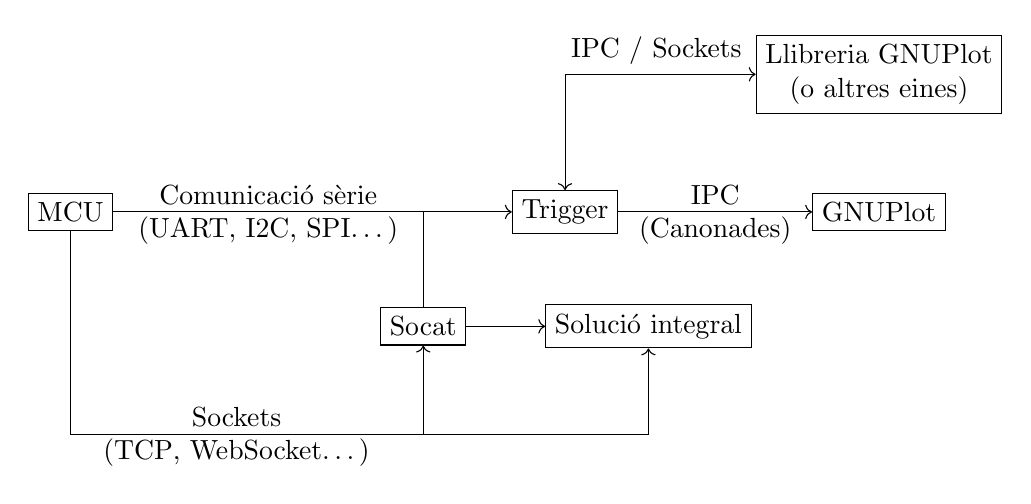
\begin{tikzpicture}
            \node[draw, rectangle] (mcu) {MCU};
            \node[right=of mcu, xshift=8em, minimum height=1.15em] (nexe-serie-socat) {};
            \node[draw, rectangle, align=center, right=of nexe-serie-socat] (trigger) {Trigger};
            \node[draw, rectangle, right=7em of trigger] (gnuplot) {GNUPlot};
            \draw[-] (mcu) -- node[yshift=-0.1em, align=center] {Comunicació sèrie\\(\acro{UART}, \acro{I2C}, \acro{SPI}\dots)} (nexe-serie-socat.center);
            \draw[->] (nexe-serie-socat.center) -- (trigger);
            \draw[->] (trigger) -- node[yshift=-0.1em, align=center] {\acro{IPC}\\(Canonades)} (gnuplot);

            \node[draw, rectangle, below=of nexe-serie-socat] (socat) {Socat};
            \node[below=of socat] (nexe-sockets) {};
            \draw[-, to path={|- node[yshift=-0.1em, xshift=6em, align=center] {\est{Sockets}\\(\acro{TCP}, WebSocket\dots)} (\tikztotarget)}] (mcu) edge (nexe-sockets.center);
            \draw[->] (nexe-sockets.center) -- (socat); \draw (socat) -- (nexe-serie-socat.center);

            \node[draw, rectangle, align=center, above=of gnuplot] (llibreria-gnuplot) {Llibreria GNUPlot\\(o altres eines)};
            \draw[-, to path={|- node[above, xshift=3.3em] {\acro{IPC} / \est{Sockets}} (\tikztotarget)}] (trigger.north) edge[<->] (llibreria-gnuplot);

            \node[draw, rectangle, align=center, right=of socat] (solucio-integral) {Solució integral};
            \node[below=of nexe-serie-socat, yshift=2.1em] (nexe-serie-solucio) {};
            \draw[->] (socat) -- (solucio-integral);
            \draw[-, to path={-| (\tikztotarget)}] (nexe-sockets.center) edge[->] (solucio-integral);
      \end{tikzpicture}
      }
\end{figure}

\section{OsPlot-MCU}

\subsection{Descripció de l'arquitectura}

OsPlot-MCU adopta un enfocament diferent per a la comunicació entre el
microcontrolador i l'ordinador. En aquest cas el programa del
microcontrolador es modifica per implementar el sistema de
\est{trigger} directament en el mateix microcontrolador.

L'avantatge principal d'aquesta solució és la seva eficiència,
especialment quan el microcontrolador té una capacitat substancial de
processament disponible. D'aquesta manera s'aprofita la totalitat dels
recursos interns del microcontrolador per realitzar el processament
necessari, reduint la càrrega computacional a l'ordinador i alliberant
recursos per altres tasques.

Precisament per això, l'enfocament d'OsPlot-MCU és adequat en
situacions en què es desitja minimitzar la càrrega computacional a
l'ordinador per diversos motius. Per exemple, en aplicacions on s'ha
de considerar l'eficiència energètica, o si es vol reduir la
dependència de l'ordinador per a tasques de processament intensives.

\subsection{Extensions}

Com amb OsPlot-PC, OsPlot-MCU ofereix altres opcions per la
comunicació entre el microcontrolador i l'ordinador. A part del port
sèrie, és possible utilitzar altres protocols de comunicació sèrie com
\acro{SPI} o \acro{I2C}, o fins i tot comunicació a través de
\est{sockets}. I també existeix la possibilitat de fer servir
llibreries específiques de GNUPlot o altres eines per fer gràfiques
com les que s'han mencionat a l'apartat
\ref{subsec:extensions-osplot-pc}.

\subsubsection{Comunicació bidireccional amb el microcontrolador}

En l'arquitectura OsPlot-MCU l'algoritme de \est{trigger} s'executa al
microcontrolador, pràcticament forçant a establir una comunicació
bidireccional per permetre l'ajust dels paràmetres del \est{trigger}.
Això vol dir que pel port sèrie circularan bytes que no representen
mostres, obligant a establir algun mecanisme per distingir-los.

Una manera senzilla i eficient d'aconseguir-ho és utilitzant un
caràcter d'escapament i enviament per paquets. Per exemple, si prenem
el byte \num{128} com a caràcter d'escapament, una mostra amb valor
\num{128} es representaria com \num{128} i \num{128}, mentre que un
final del paquet de mostres es pot indicar amb els bytes \num{128} i
\num{0}. Altres maneres més elaborades impliquen l'ús d'eines com
\href{https://protobuf.dev/}{\underline{Protobuf}}, un mecanisme
eficient de serialització que permet estructurar dades per crear un
protocol de comunicació.

\newpage

\subsection{Diagrama de l'arquitectura}

\begin{figure}[!hb]
      \centering
      \resizebox{\textwidth}{!}{
      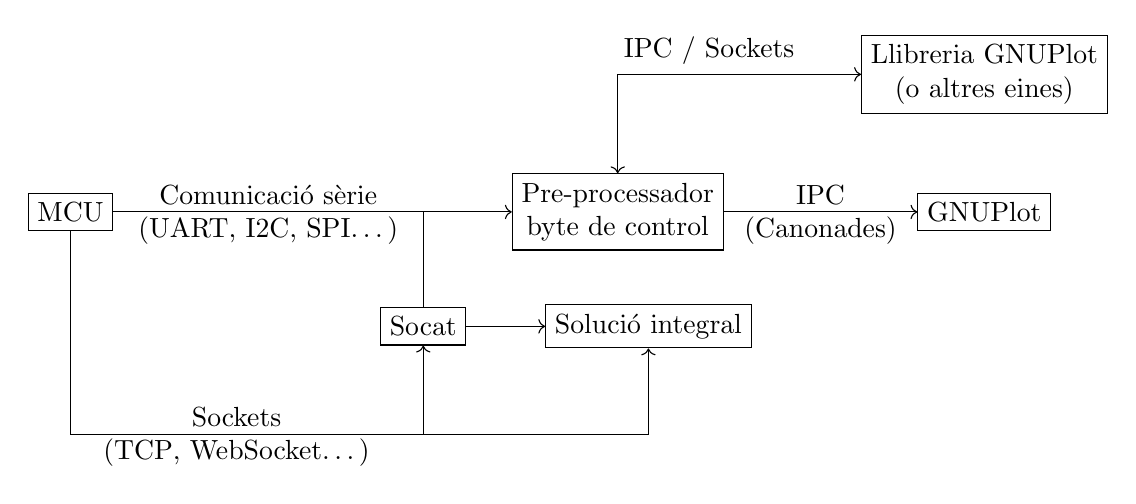
\begin{tikzpicture}
            \node[draw, rectangle] (mcu) {MCU};
            \node[right=of mcu, xshift=8em, minimum height=1.15em] (nexe-serie-socat) {};
            \node[draw, rectangle, align=center, right=of nexe-serie-socat] (trigger) {Pre-processador\\byte de control};
            \node[draw, rectangle, right=7em of trigger] (gnuplot) {GNUPlot};
            \draw[-] (mcu) -- node[yshift=-0.1em, align=center] {Comunicació sèrie\\(\acro{UART}, \acro{I2C}, \acro{SPI}\dots)} (nexe-serie-socat.center);
            \draw[->] (nexe-serie-socat.center) -- (trigger);
            \draw[->] (trigger) -- node[yshift=-0.1em, align=center] {\acro{IPC}\\(Canonades)} (gnuplot);

            \node[draw, rectangle, below=of nexe-serie-socat] (socat) {Socat};
            \node[below=of socat] (nexe-sockets) {};
            \draw[-, to path={|- node[yshift=-0.1em, xshift=6em, align=center] {\est{Sockets}\\(\acro{TCP}, WebSocket\dots)} (\tikztotarget)}] (mcu) edge (nexe-sockets.center);
            \draw[->] (nexe-sockets.center) -- (socat); \draw (socat) -- (nexe-serie-socat.center);

            \node[draw, rectangle, align=center, above=of gnuplot] (llibreria-gnuplot) {Llibreria GNUPlot\\(o altres eines)};
            \draw[-, to path={|- node[above, xshift=3.3em] {\acro{IPC} / \est{Sockets}} (\tikztotarget)}] (trigger.north) edge[<->] (llibreria-gnuplot);

            \node[draw, rectangle, align=center, right=of socat] (solucio-integral) {Solució integral};
            \node[below=of nexe-serie-socat, yshift=2.1em] (nexe-serie-solucio) {};
            \draw[->] (socat) -- (solucio-integral);
            \draw[-, to path={-| (\tikztotarget)}] (nexe-sockets.center) edge[->] (solucio-integral);
      \end{tikzpicture}
      }
\end{figure}

\chapter{Implementació d'OsPlot-PC amb Arduino-C/Python/Chart.js}

En aquesta secció es descriu un exemple d'implementació
d'OsPlot-PC. El programa de l'Arduino és el mateix que s'ha descrit a
l'apartat \ref{programa-arduino-c}. L'algoritme de \est{trigger}
s'implementarà utilitzant Python asíncron, i es comunicarà amb una
interfície basada en tecnologia web mitjançant l'ús de WebSockets.

El codi font d'aquesta implementació es pot trobar a
\url{https://github.com/JoanVC100/OsPlot/tree/main/OsPlot-PC}.

\section{\est{Trigger} Python amb WebSockets}

\subsection{Descripció de l'algoritme de \est{trigger}}
\label{subsec:maquina-trigger}

Per simplicitat, s'ha modelat mitjançant una màquina d'estats un
algoritme de ``\est{trigger} normal'' activat per flanc de pujada
(sense disparador automàtic).

La màquina comença en l'estat ``ESPERANT\_TRIGGER'', on compara
successivament les mostres d'entrada amb un nivell de \est{trigger}
predefinit. Quan es detecta un flanc de pujada (la mostra anterior és
inferior o igual al nivell de \est{trigger}, i la mostra actual és
igual o superior al nivell de \est{trigger}), la màquina passa a
l'estat ``CAPTURANT''.

En l'estat de ``CAPTURANT'' es fa servir un comptador que disminueix a
mesura que arriben les mostres. Un cop es captura un nombre de mostres
determinat (n\_capturades $== 0$), s'envien les mostres a la
interfície i la màquina torna a l'estat d'``ESPERANT\_TRIGGER''.

\begin{figure}[!hb]
      \centering
      \resizebox{\textwidth}{!}{
      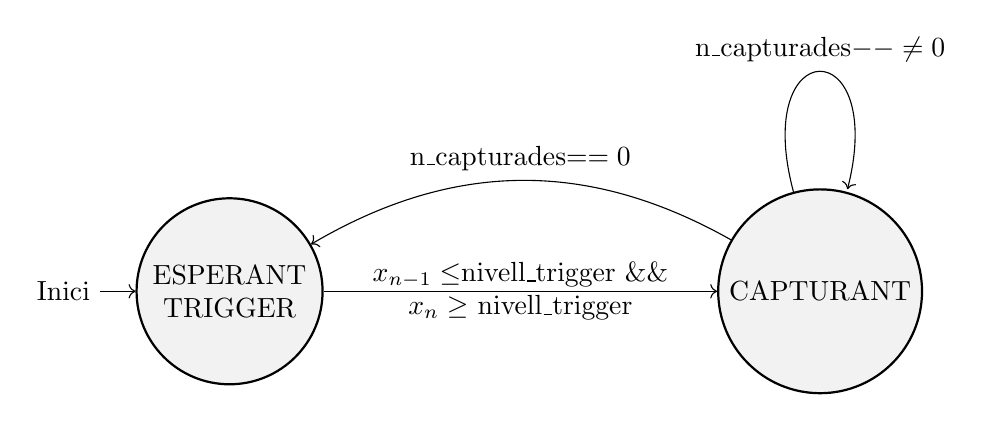
\begin{tikzpicture}[node distance=7.5cm]
            \node[state, initial, align=center] (esperant_trigger) {ESPERANT\\TRIGGER};
            \node[state, right of=esperant_trigger] (capturant) {CAPTURANT};
            \draw (esperant_trigger) edge[->] node[align=center]{$x_{n-1}\leq$nivell\_trigger \&\&\\$x_{n}\geq$ nivell\_trigger} (capturant)
            (capturant) edge[loop above] node[align=center]{n\_capturades$--\neq 0$} (capturant)
            (capturant) edge[bend right, above, ->] node[align=center]{n\_capturades$== 0$} (esperant_trigger);
      \end{tikzpicture}
      }
      \caption{Diagrama de la màquina d'estats del \est{trigger}}
\end{figure}

\subsection{Transmissió de les mostres amb WebSockets}

Els \cite[WebSockets]{websockets} són una tecnologia que permet una
comunicació persistent, bidireccional i en temps real entre client i
servidor. Aquesta tecnologia és ideal per rebre les mostres del
\est{trigger} i alhora comunicar-se amb el servidor per canviar certs
paràmetres de l'algoritme. En aquest projecte, s'ha utilitzat la
llibreria de Python
\href{https://pypi.org/project/websockets/}{\underline{websockets}},
que està dissenyada per treballar amb Python asíncron
(\href{https://docs.python.org/3/library/asyncio.html}{\underline{asyncio}}).

Primerament, el programa de \est{trigger} ha de cridar a la funció
\ord|websocket.serve()|, que crea un servidor WebSocket per acceptar
peticions de connexions (escoltant al port 26142), i hi associa una
funció que s'executarà per cada connexió entrant.

Aquesta funció afegeix cada connexió en un conjunt global de Python
(un \est{set} global) i entra en un bucle infinit. Dins del bucle
principal, s'encarrega de rebre i gestionar els missatges enviats pels
usuaris, com ara les so\l.licituds de canvi de paràmetres específics.

D'altra banda, la màquina d'estats del \est{trigger} fa servir el
conjunt de connexions global per realitzar un \est{broadcast} de les
mostres quan la màquina surt de l'estat ``CAPTURANT'', enviant de
manera efectiva les mostres a tots els clients connectats a través de
WebSockets.

I per simplificar la comunicació entre la interfície i el
\est{trigger} s'ha utilitzat Protobuf, que permet canviar els
paràmetres de l'algoritme de \est{trigger} i rebre dades del servidor,
com les mostres capturades. Protobuf fa servir un format de missatges
estructurat i eficient ($\approx 2$ bytes de sobrecàrrega per paquet de
mostres), mantenint una transmissió de dades lleugera pels clients.

\section{Interfície amb Chart.js}

La interfície per visualitzar les mostres de l'osci\l.loscopi s'ha
desenvolupat utilitzant tecnologia web, fet que permet aprofitar els
avantatges d'entorns com Tauri per crear aplicacions multiplataforma.

Per la construcció dels gràfics en temps real s'ha utilitzat una
llibreria JavaScript anomenada Chart.js. Aquesta llibreria aprofita
l'element \est{canvas} de HTML5 que ofereix una experiència visual
atractiva i interactiva, alhora que manté un bon rendiment respecte
a altres alternatives.

A diferència de GNUPlot, es transfereixen directament les mostres a
una matriu associada al gràfic (en comptes de fer servir
cues). Aquesta matriu conté les dades dels eixos $x$ i $y$. Quan
arriba un paquet de mostres a través del WebSocket, es copien totes
les mostres a les $y$ i es crida la funció \ord|update()| per
actualitzar el gràfic amb les noves dades.

\begin{figure}[h]
  \centering 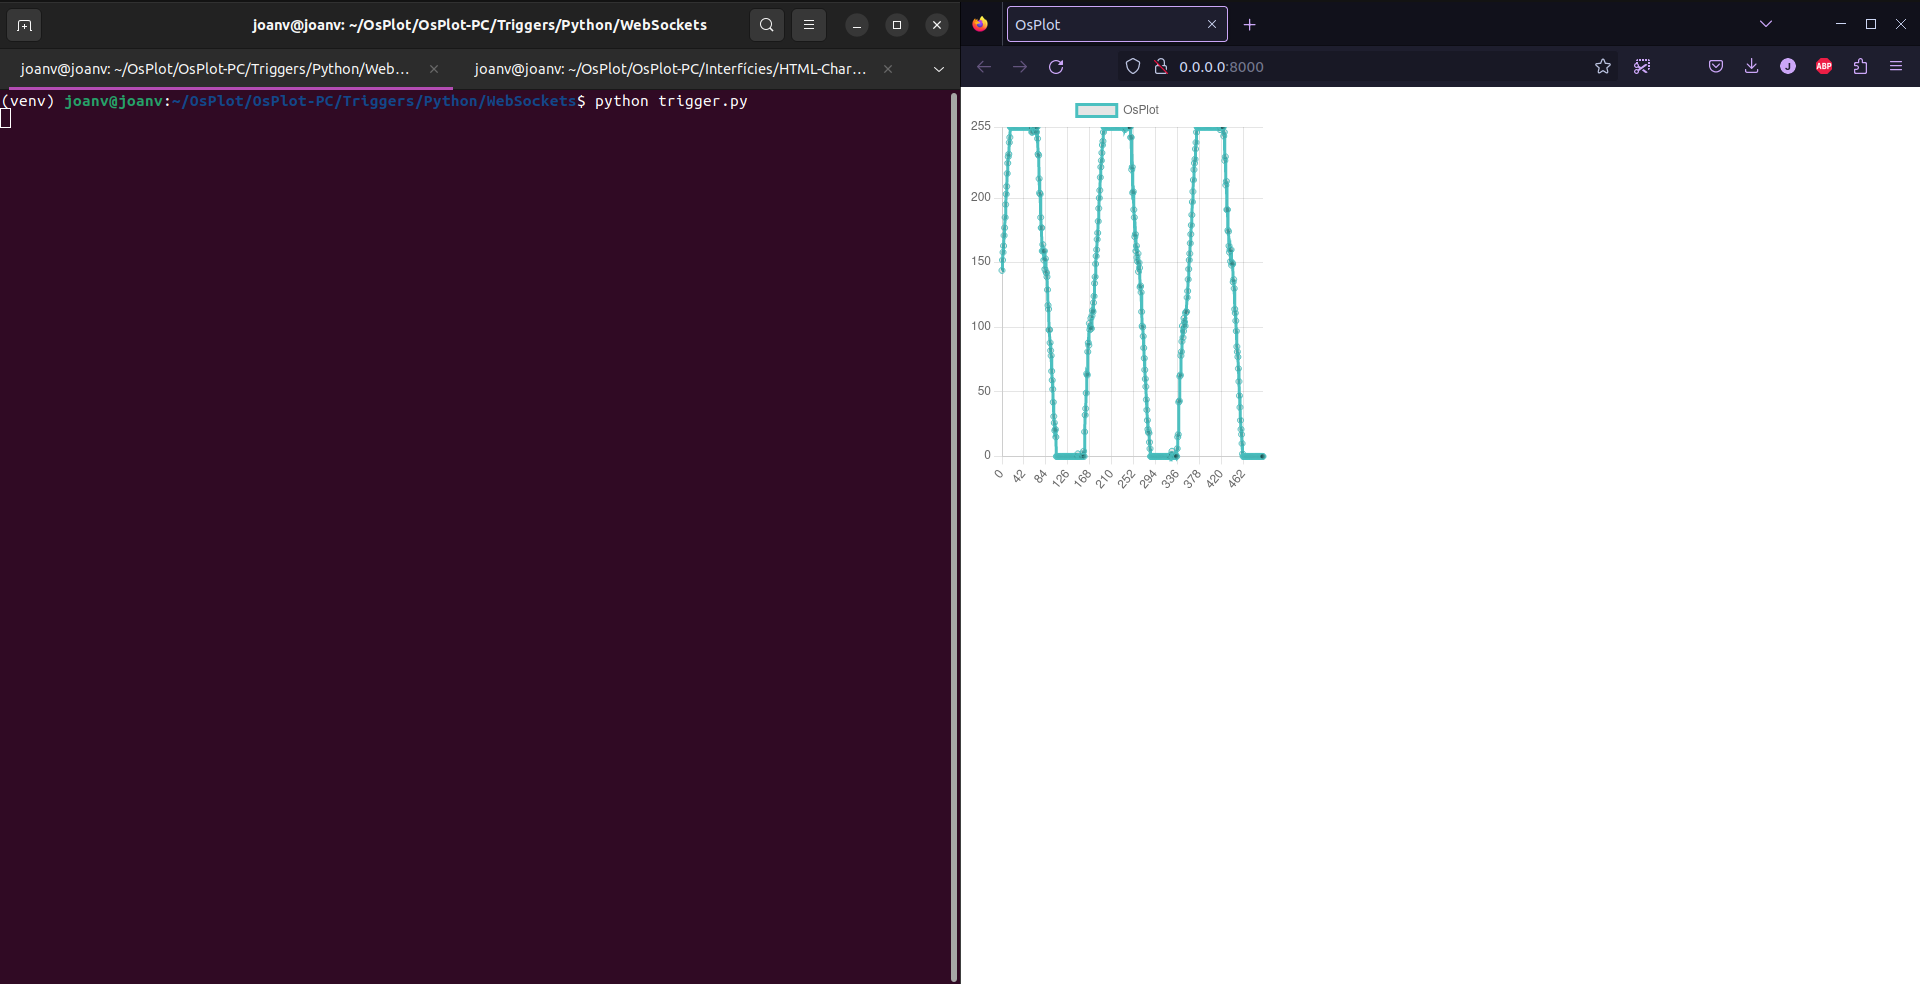
\includegraphics[width=\textwidth]{imgs/OsPlot-PC.png}
  \caption{Captura de l'implementació d'OsPlot-PC}
\end{figure}

\chapter{Implementació d'OsPlot-MCU amb Arduino-C/Rust/GNUPlot}

\section{Modificació del programa d'Arduino}

Com a punt de partida, es prendrà el programa desenvolupat a l'apartat
\ref{programa-arduino-c} i s'hi incorporarà la màquina d'estats de
l'apartat \ref{subsec:maquina-trigger} mitjançant un bucle després
d'inicialitzar els perifèrics. A més, s'afegirà la comunicació
bidireccional per permetre canviar els paràmetres del \est{trigger}
des de la interfície, mitjançant una altra màquina d'estats. I per
acabar, s'inclourà un filtre per reduir la freqüència de mostreig
efectiva calculant una mitjana de $n$ mostres per tal de reduir el
soroll que captura l'\acro{ADC}.

El codi font d'aquesta implementació es pot trobar a
\url{https://github.com/JoanVC100/OsPlot/tree/main/OsPlot-MCU}.

\subsection{Comunicació bidireccional amb el \est{trigger}}

Per a la comunicació bidireccional, s'ha adoptat una estratègia basada
en l'enviament de paquets amb bytes de control per minimitzar el temps
processament de mostres. S'ha implementat una màquina d'estats que, en
l'estat ``MÀQUINA\_TRIGGER'', continua llegint mostres mentre no es
generi una interrupció de recepció de bytes.

Però, quan es produeix la primera interrupció, es para la captura de
mostres i l'Arduino queda en l'estat ``REBRE\_ORDRES'', en espera
d'ordres de l'ordinador. Només es reactiva l'algoritme de
\est{trigger} quan s'envia l'ordre ``INICIA\_TRIGGER'' des de
l'ordinador.

\begin{figure}[!hb]
      \centering
      \resizebox{\textwidth}{!}{
      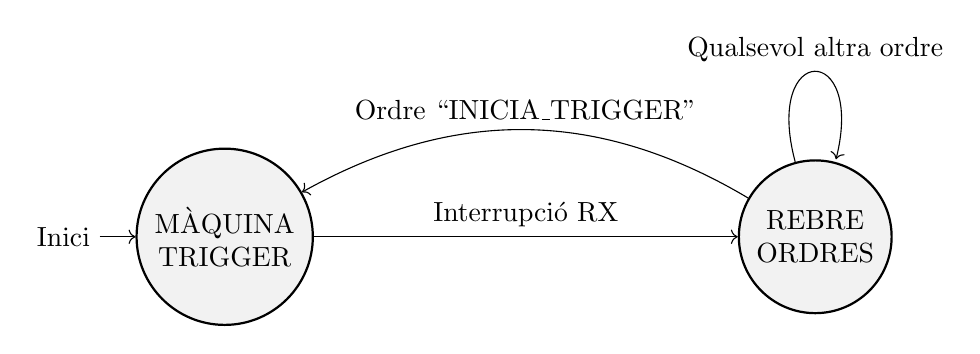
\begin{tikzpicture}[node distance=7.5cm]
            \node[state, initial, align=center] (maquina_trigger) {MÀQUINA\\TRIGGER};
            \node[state, right of=maquina_trigger, align=center] (rebre_ordres) {REBRE\\ORDRES};
            \draw (maquina_trigger) edge[->, above] node{Interrupció RX} (rebre_ordres)
            (rebre_ordres) edge[loop above] node{Qualsevol altra ordre} (rebre_ordres)
            (rebre_ordres) edge[bend right, above, ->] node{Ordre ``INICIA\_TRIGGER''} (maquina_trigger);
      \end{tikzpicture}
      }
      \caption{Diagrama de la màquina d'estats per la comunicació bidireccional}
\end{figure}

\clearpage

El protocol de comunicació bidireccional utilitza un byte de control
amb valor \num{128} seguits d'un byte que indica el tipus de missatge
enviat:

\begin{itemize}
\item MCU\_FINESTRA: Indica el final d'un paquet de mostres. Pot tenir
  qualsevol mida.
\item MCU\_FACTOR\_OVERSAMPLING\_CANVIAT: Indica èxit en canviar el
  nombre de mostres del filtre de mitjana.
\item MCU\_FACTOR\_OVERSAMPLING: És un paquet que conté un byte amb el
  nombre de mostres del filtre de mitjana.
\item MCU\_N\_MOSTRES\_CANVIADES: Indica que el nombre de mostres
  d'una finestra s'ha canviat.
\item MCU\_N\_MOSTRES: Paquet que conté el nombre de mostres d'una
  finestra (2 bytes).
\item MCU\_FS: Retorna la freqüència de mostreig de l'\acro{ADC}. És
  un real de \num{4} bytes.
\item MCU\_NIVELL\_TRIGGER\_CANVIAT: Indica que el nivell del
  \est{trigger} s'ha canviat.
\item MCU\_NIVELL\_TRIGGER: Retorna un byte amb el nivell de
  \est{trigger}.
\item MCU\_ERROR: Aquest missatge indica que s'ha produït un error en
  la comunicació amb l'Arduino. Pot ser causat per una comanda
  incorrecta, valors invà\l.lids\dots
\end{itemize}

\subsection{Filtre per reduïr la freqüència de mostreig efectiva}

La implementació del filtre per reduir la freqüència de mostreig
efectiva utilitza una tècnica de mitjana de $n$ mostres. Aquesta
tècnica permet reduir el soroll capturat per l'\acro{ADC} disminuint
la freqüència de mostreig efectiva. La freqüència efectiva es calcula
dividint la freqüència de mostreig original pel nombre de mostres
usades en el càlcul de mitjana ($\frac{F_{s}}{n}$).

Aquest tractament del senyal pot ser útil quan es vol visualitzar
senyals de més baixa freqüència amb més resolucio (> \SI{8}{\bits}), o
com a mètode per augmentar les divisions de temps. Però és important
tenir en compte que aquesta mitjana pot tenir un efecte negatiu en la
captura de pics ràpids. El suavitzat de les fluctuacions pot
provocar que els pics ràpids es redueixin o desapareguin a la
representació gràfica. Aquesta és una limitació inherent de la tècnica
de mitjana, i s'hauria de solucionar amb altres enfocaments, com el
\est{trigger} amb detecció de pics.

\section{Programa auxiliar amb Rust}

El programa d'OsPlot-MCU escrit en Rust està orientat a la programació
asíncrona i per esdeveniments. S'utilitza tokio, una biblioteca de
programació asíncrona per al llenguatge Rust. Proporciona eines i
abstraccions per gestionar aquesta tècnica de programació de manera
senzilla. En concret es fa servir l'extensió tokio-serial, que afegeix
la possibilitat d'interactuar amb ports sèrie asíncronament.

\newpage

La tasca principal del programa és una funció que, primer de tot,
inicialitza el port sèrie enviant la comanda per iniciar el
\est{trigger} del microcontrolador. Seguit d'això, es crea el procés
de GNUPlot en un directori temporal, que conté la cua per la
transmissió de mostres i el \est{script} que ha d'executar. Aquest
\est{script} inclou alguna modificació, ja que els valors de l'eix $x$
s'envien també per la cua, evitant a GNUPlot càlculs per cada
representació.

Aquesta tasca entra en un bucle que contínuament llegeix paquets del
port sèrie. Quan arriba un paquet de mostres, les mostres es copien a
una matriu que contindrà cada mostra i la seva corresponent $x$, i
l'enviarà directament a través de la canonada (per la resta de
paquets no es realitza accions rellevants). Aquest bucle només podrà
acabar quan, o bé hi hagi algún error (es tanca el port sèrie, mor
el procés de GNUPlot\dots), o si la tasca de la \acro{CLI} li envia
un missatge de tancament (per Ctrl-C, ordre de sortida\dots).

La tasca de la \acro{CLI} té com a funció interpetar ordres de
l'usuari (que arriben per \fitx{stdin}) i transmetre-les a la tasca
principal.  Per limitacions de tokio, en comptes de crear una tasca
per llegir la \fitx{stdin}, es crea un fil que llegeix l'entrada de
l'usuari i l'envia a la tasca de la \acro{CLI}. I per gestionar el
Ctrl-C, es crea un altre fil que envia una senyal a la mateixa tasca.

Tota la comunicació entre tasques és possible gràcies als \acro{MPSC}
(\est{Multi-Producer Single-Consumer}) i \est{Oneshots}, que són
canals asíncrons que permeten la comunicació entre múltiples
tasques. Separar el programa en aquestes tasques permet separar els
diferents blocs d'esdeveniments d'una manera clara i estructurada.

\begin{figure}[h]
  \centering 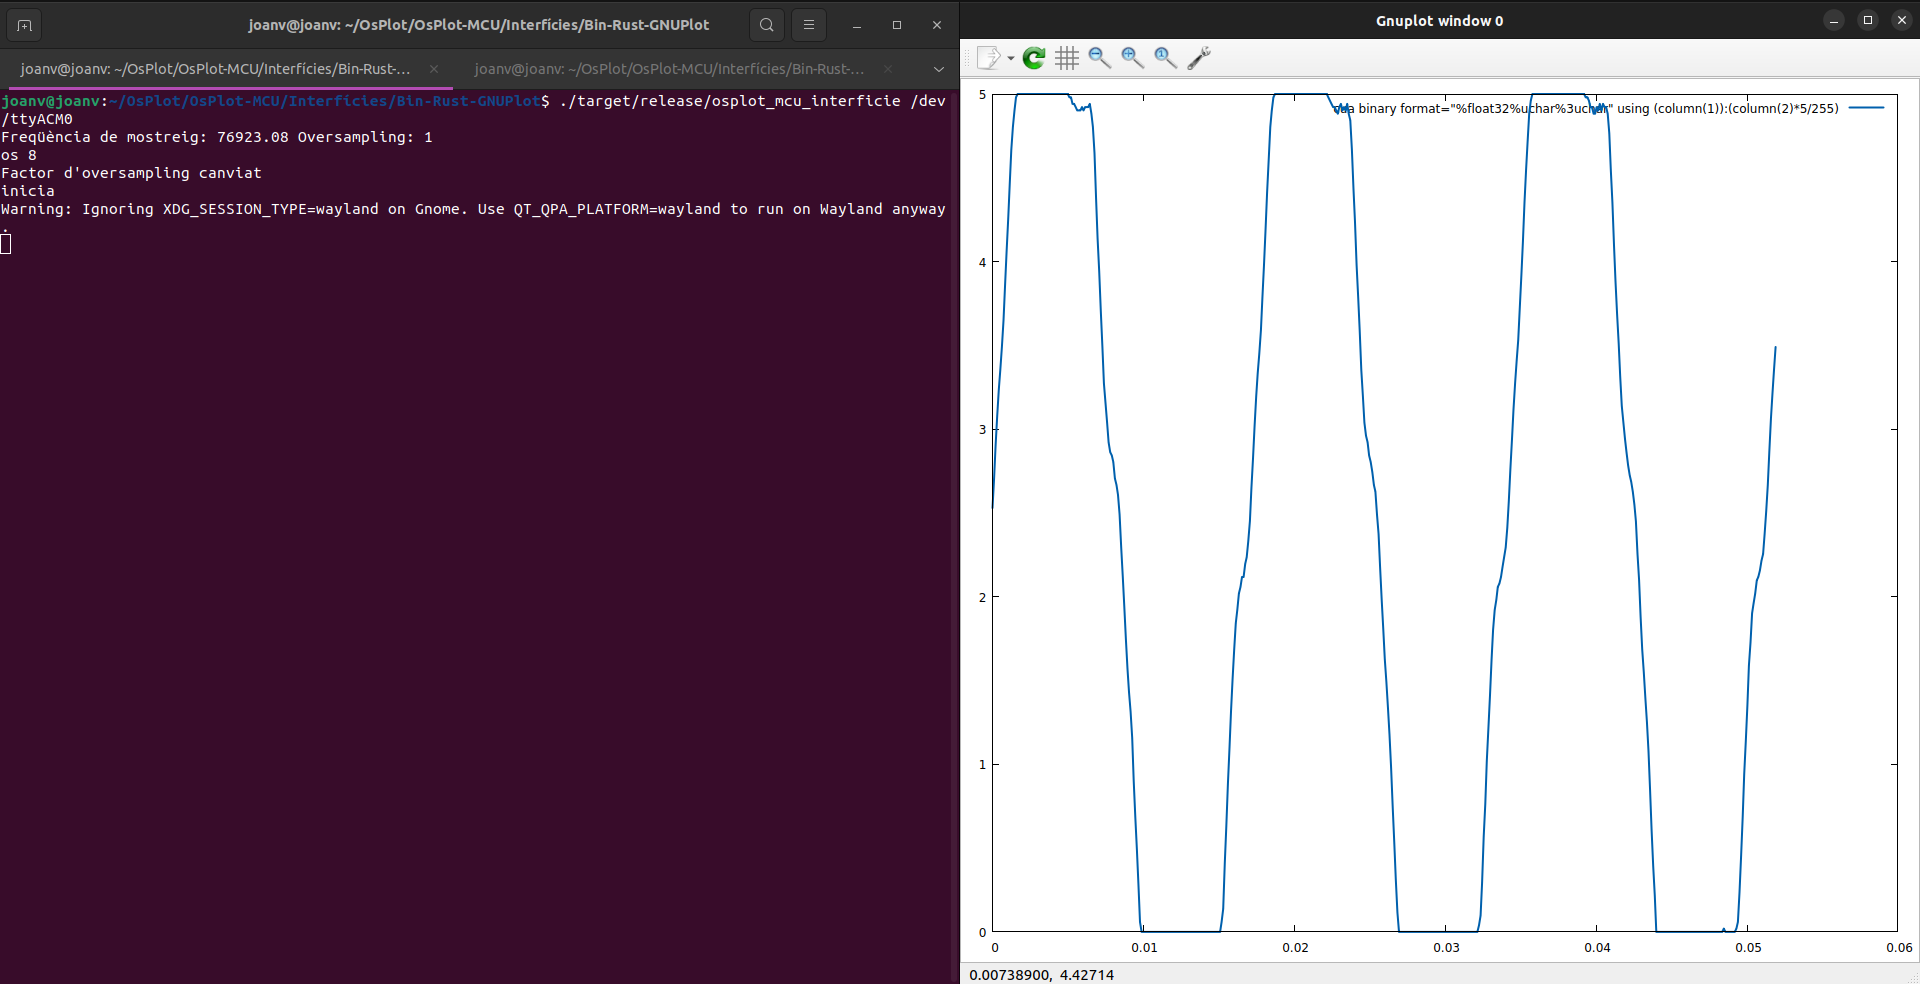
\includegraphics[width=\textwidth]{imgs/OsPlot-MCU.png}
  \caption{Captura de l'implementació d'OsPlot-MCU}
\end{figure}

\chapter{Línies futures}

\section{Múltiples esdeveniments de \est{triggers} per \est{frame}}

En buscar la simplicitat, les implementacions realitzades en el
treball no tenen en compte la visualització de múltiples esdeveniments
de \est{trigger} en un únic \est{frame}. Tota informació que no pugui
ser representada en el transcurs de dos \est{frames} consecutius es
descarta. Això significa que, en casos on la freqüència del senyal és
alta i hi ha una gran quantitat d'esdeveniments de \est{trigger} per
temps de \est{frame}, l'observador pot perdre moltes dades rellevants
i no ser capaç de discernir tots els esdeveniments que s'han produït
en el transcurs d'un \est{frame}.

Els osci\l.loscopis professionals tenen en compte aquesta limitació i
implementen solucions per superar-la. Un enfocament comú és utilitzar
una representació visual que permet mostrar tots els disparaments
generats en el transcurs d'un \est{frame} determinat. Aquesta tècnica
implica assignar una transparència variable als esdeveniments de
\est{trigger}, de manera que les ones més antigues apareguin més
transparents, mentre que les ones més recents es mostren més clares i
destacades. Aquesta representació visual proporciona una indicació de
la forma i la tendència del senyal al llarg del temps sense augmentar
la capacitat de visualització de la pantalla.

Amb aquesta tècnica, l'observador pot identificar si hi ha hagut
picades o canvis significatius en el senyal durant el \est{frame},
així com observar si el senyal és estable o no. Aquesta informació és
valuosa per a l'anàlisi i la comprensió del comportament del senyal en
situacions en què hi ha múltiples esdeveniments de \est{trigger} en un
període de temps que la pantalla de l'osci\l.loscopi no podria
representar (o fins i tot, que l'ull humà no podria apreciar).

\section{Plantejar alternatives al port sèrie}

En el marc d'aquest treball, s'ha observat que es pot arribar
ràpidament al límit de velocitat del port sèrie. Amb una taxa
d'\acro{ADC} estable d'aproximadament \num{76000} mostres per segon,
utilitzar una velocitat de transmissió d'\SI{1}{\mega\bit\per\second}
(\num{100000} mostres per segon) comença a ser insuficient per
acomodar el flux de dades de l'osci\lgem oscopi. Si es pogués
augmentar la velocitat de mostreig de l'\acro{ADC} a l'Arduino, el
port sèrie deixaria de ser una opció viable, ja que una velocitat de
\SI{2}{\mega\bit\per\second} resultaria molt més inestable que
\SI{1}{\mega\bit\per\second} (velocitat la qual ja està fora de
l'estàndard).

En vista d'aquesta limitació, cal explorar alternatives. Per exemple,
es podria fer servir \acro{SPI}, que permet una velocitat màxima de
fins a 60 Mbps en alguns casos, sense experimentar una càrrega
excessiva. Això implicaria un augment significatiu en la taxa de
mostreig teòrica, arribant a un màxim de \num[round-precision=1]{7.5}
milions de mostres per segon.

Una altra opció a considerar seria buscar mètodes de comunicació
directa a través de la interfície \acro{USB}, evitant conversions de
port sèrie a \acro{USB} i a l'inrevés (com és el cas de l'Arduino). El
programa a l'ordinador podria accedir directament a l'\acro{USB},
augmentant molt més les velocitats de transmissió teòriques, segons
l'estàndard \acro{USB} utilitzat.

\section{Inclusió de les \acro{SDR} a l'arquitectura}

Una altra línia futura interessant a explorar és l'ús de la \cite[Ràdio
  Definida per Software]{viqui-sdr}. En lloc d'utilitzar protocols
serials com \acro{UART} o \acro{SPI}, o altres tecnologies
de xarxa com \acro{TCP/IP} o WebSockets, l'ús de una \acro{SDR}
pot proporcionar una solució més versàtil per a la lectura, el
processament i l'enviament de mostres.

Les \acro{SDR} són dispositius que permeten capturar, processar i
transmetre senyals de ràdio mitjançant programari. A diferència dels
sistemes de ràdio tradicionals, que utilitzen components electrònics
especialitzats per a funcions específiques, les \acro{SDR} es basen en
plataformes programables i flexibles que utilitzen processament
digital de senyals per dur a terme diverses tasques de comunicació.
Mitjançant l'ús de programari és possible canviar i adaptar els
paràmetres i funcions de les \acro{SDR}, com la modulació, la
freqüència i la codificació, per adaptar-se a diferents aplicacions i
requisits.

S'hauria d'investigar com integrar-los a l'arquitectura OsPlot per
intentar aprofitar les seves capacitats de processament digital. Una
\acro{SDR} permet capturar senyals analògics, convertir-los en senyals
digitals i processar-los mitjançant algoritmes de processament de
senyal digital. Això obriria la porta a una gran varietat de tècniques
de modulació, codificació i descodificació que podrien ser utilitzades
per a la transmissió de mostres. També es podria investigar l'ús de
diferents bandes de freqüència per a una millor transmissió de les
mostres, etc\dots

\chapter{Conclusions}

El treball de final de grau ha aconseguit complir amb èxit els
objectius establerts. En primer lloc, s'ha avaluat de manera
exhaustiva la capacitat de GNUPlot per a la visualització de dades
en temps real. S'ha pogut demostrar de múltiples maneres que,
sense modificacions addicionals, GNUPlot pot funcionar en temps real
d'una manera prou eficient.

En segon lloc, s'ha desenvolupat amb èxit una guia que descriu una
arquitectura capaç de transformar un microcontrolador i un ordinador
en un osci\l.loscopi funcional. L'arquitectura ha estat implementada
de manera modular i flexible, permetent adaptar-se a diferents
microcontroladors i entorns de treball.

A més, s'han realitzat implementacions de referència que exploren les
diferents possibilitats de l'arquitectura OsPlot. Aquestes
implementacions engloben des de la més bàsica fins les més complexes.

La implementació bàsica ha estat un pas important per destacar la
simplicitat que pot tenir l'arquitectura. Amb aquesta implementació es
buscava dur a terme la transmissió de mostres des del microcontrolador
a GNUPlot mitjançant una canonada simple, permetent la visualització i
l'anàlisi del senyal en temps real.

D'altra banda, les implementacions més complexes han posat de manifest
la versatilitat de l'arquitectura OsPlot en escenaris d'aplicació més
exigents. Amb suport per algoritmes de \est{trigger}, s'ha
possibilitat la captura i visualització selectiva de determinats
esdeveniments o patrons en el senyal. I la possibilitat d'utilitzar
altres mètodes per transmetre les mostres, com \acro{SPI}, WebSockets
o \acro{SDR}, obre un ventall de possibilitats per a la transferència
ràpida de grans volums de mostres.

Finalment, s'ha aconseguit ajuntar l'arquitectura OsPlot amb altres
alternatives a GNUPlot (com ploterrs o Chart.js). Això permet als
usuaris a estendre l'arquitectura amb altres eines de visualització de
dades, adaptant-se a les seves necessitats i preferències.

En resum, el treball d'aquest document serveix com una guia valuosa per
transformar un microcontrolador i un ordinador en un osci\l.loscopi
digital totalment funcional, amb múltiples variants i funcionalitats.
S'han complert els objectius plantejats, i s'ha proporcionat una base
sòlida per a futures investigacions i desenvolupaments en aquest
àmbit.

\printbibliography

\end{document}

%%% Local Variables:
%%% mode: latex
%%% TeX-master: t
%%% LaTeX-biblatex-use-Biber: t
%%% End:
